\chapter{Improvements to the Weather Research and Forecasting Model over First-Year Sea Ice}
\vspace{1 cm}
\begin{spacing}{1} \begin{quote} 
\noindent \emph{Current Arctic sea ice coverage levels (both annual and late summer) are at their lowest since at least 1850 (high confidence), and for late summer for the past 1000 years (medium confidence). Since the late 1970s, Arctic sea ice area and thickness have decreased in both summer and winter, with sea ice becoming younger, thinner and more dynamic (very high confidence).}\end{quote}
\hspace{6 cm} - IPCC Sixth Assessment Report, August 2021  
\end{spacing}
\doublespacing
\section{Introduction}

Models in the polar regions have the largest uncertainties relative to other parts of the Earth \citep{holland:2003, AACI:05}. Models have difficulty simulating radiation accurately during times of thick clouds. A likely reason for this is the model’s inability to estimate the fraction of liquid water within the cloud \citep{graham:2017}. A surface inversion often persists during the winter months and processes under these stable conditions are not well understood or modeled \citep{tastula:2012}. In the summer, these inversions are often elevated compared to the wintertime surface inversions \citep{serreze:1992}. Models, however, are integral for understanding the processes occurring in the polar regions, particularly the radiation. Unfortunately, few field experiments collecting data for validation exist.
 
Reanalysis products are often used to study Arctic climate. This poses a challenge as they are not as thoroughly verified as in other locations due to the extreme climate and harsh winter conditions preventing accurate, long-term, multi-season, in-situ measurements. Biases in clouds result in difficulties in resolving the surface energy budget. Recent studies have shown that when compared with surface observations, reanalysis have large biases in cloud properties (liquid/ice water path, fraction). A number of field experiments have shown that mixed-phase clouds are dominant in autumn through spring in the lower levels at high latitudes \citep{intrieri:2002, wang:2005}. Cloud micro- and macrophysics are closely tied to the surface energy budget, but cloud parameterizations are not well developed in models for the polar regions. Particularly in the Arctic, the radiative properties of clouds and how they are parameterized in models are of importance to modeling the surface energy budget.
 
The Norwegian Young Sea Ice Experiment (N-ICE) field campaign described in Chapter 2 was the first winter field experiment in the Arctic since the Surface Heat Budget of the Arctic (SHEBA) experiment, taking place onboard a research vessel frozen into Arctic sea ice. SHEBA’s primary goals were to observe the surface energy budget, ice mass balance, and ocean-ice-atmosphere interactions in the Arctic during a year-long period from October 1997 to October 1998. Much like N-ICE, SHEBA was motivated by changes in the Arctic and the need for a better understanding of physical processes in the polar regions \citep{randall:1998}. A secondary objective of SHEBA was to improve model simulations of the Arctic for use in global climate models \citep{uttal:2002}. Both the ice-albedo feedback and the cloud-radiation feedback were extensively studied using datasets collected during this field experiment. However, this experiment occurred 18 years prior to N-ICE and in a different location of the Arctic, influenced by different synoptic conditions. 

 As described in Chapter 3 of this dissertation, results showed that WRF-Polar does not accurately simulate conditions observed at N-ICE, regardless of the boundary-layer and cloud microphysics scheme selected. Chapter 4 explored the cloud radiative forcing and found that mixed-phase clouds were present throughout much of the observation period. This chapter also compared the calculated cloud radiative forcing to that observed at N-ICE and found that the cloud influence on radiation was not accurately represented in the model, particularly in the shortwave. Chapter 5 expanded on the previous chapters by looking specifically at how well equations to estimate flux do under the conditions at N-ICE. This chapter was motivated by the previous two chapters with the goal of determining if the error in the model could be reduced by improving the equations used to estimate flux. Fixing the cloud-induced error in the latent and sensible heat flux equations is impossible without first knowing how much error the equation itself introduces when the correct radiation is input.

This chapter focuses on improving two parts of the model: the use of more appropriate surface properties for thin sea ice and the equations used to estimate flux in the land surface model. Two separate sensitivity studies are presented here. The first explores the sensitivity of surface properties by changing values within a lookup table used by the WRF model related to the land surface. This study uses the N-ICE observations to select improved values for thin sea ice. The second sensitivity study uses the turbulent flux equations described in Chapter 5 to compare different methods for estimating sensible and latent heat fluxes. This chapter concludes by making recommendations as to which flux equations perform the best for simulations over young, thin sea ice.

\section{Methods}
The idealized version of the Weather Research and Forecasting model \citep{skamarock:2019} was used to test the sensitivity of the model to changes in the set of parameters found in the model's land use table, LANDUSE.TBL. The idealized version of WRF is different from the ``real" version used in Chapter 3 and in forecasts. The idealized version simplifies the model by removing the effects of advection and topography. Idealized model simulations are used only in research as they create an ``idealized" atmosphere at a point in space. These simulations are not as computationally expensive or as time-consuming as running the full WRF model and are used to isolate specific parts of the model for sensitivity testing \citep{arw:2019}. 

The LANDUSE.TBL file is one of three tables used in WRF to set constants. This file specifies constants that pertain to the surface-atmosphere interface within the model, including the surface albedo, surface moisture availability, surface emissivity, surface roughness, thermal inertia constant, snow cover effect, and surface heat capacity. There are different ``sections" within this table. Much like choosing different physical schemes based on expected conditions, these sections each have sets of values that were determined from various experiments, and the sections typically specify values for summer and winter separately. 

The values in this table are generally empirically derived or directly measured from field experiments. The classification for sea ice is very general as it encompasses all permanent or seasonal snow and ice surfaces and uses one set value for each variable defined in this table for all snow surface conditions. The only exception to this is the albedo. The user has the option to specify the albedo in the file used to start the model. However, doing this will only specify one albedo value. The LANDUSE.TBL values generally give different values for summer and winter, so there is an advantage to letting LANDUSE.TBL set these values during long runs. 

\begin{table}[t]
\footnotesize
\center
\centering
\doublespacing
\begin{tabular}{| c | c | c | c | c |  c |}
\hline
 \rowcolor[HTML]{ECECEC} \rule{0pt}{35pt} \multirow{-2}{*}{\textbf{Section}} & \multirow{-2}{*}{\textbf{Season}} & \multirow{-2}{*}{\textbf{\shortstack{Albedo\\ $(\%)$}}} & \multirow{-2}{*}{\textbf{\shortstack{Surface \\ Emissivity\\ $(\%)$}}} & \multirow{-2}{*}{\textbf{\shortstack{Roughness Length}}} & \multirow{-2}{*}{\textbf{Category}} \\ \hline
\rule{0pt}{12pt} & Summer & 55 & 95 & 5 &  \\
\rule{0pt}{12pt} \multirow{-2}{*}{\textbf{OLD}} & Winter & 70 & 95 & 5 & \multirow{-2}{*}{\shortstack{Permanent \\ Ice}} \\ \hline
\rule{0pt}{12pt} & Summer & 55 & 95 & .1 &  \\
\rule{0pt}{12pt} \multirow{-2}{*}{\textbf{USGS}} & Winter & 70 & 95 & .1 & \multirow{-2}{*}{\shortstack{Snow or Ice}} \\ \hline
\rule{0pt}{12pt} & Summer & 55 & 95 & .1 &  \\
\rule{0pt}{12pt} \multirow{-2}{*}{\textbf{\shortstack{MODIFIED IGBP \\ MODIS NOAH}}} & Winter & 70 & 95 & .1 & \multirow{-2}{*}{\shortstack{Snow or Ice}} \\ \hline
\rule{0pt}{12pt} & Summer & 55 & 95 & 5 &  \\
\rule{0pt}{12pt}\multirow{-2}{*}{\textbf{SiB}} & Winter & 70 & 95 & 5 & \multirow{-2}{*}{\shortstack{Ice Cap \\ and Glacier}} \\ \hline
\rule{0pt}{12pt} & Summer & 55 & 95 & 1 &   \\
\rule{0pt}{12pt}\multirow{-2}{*}{\textbf{MODIS}} & Winter & 55 & 98 & 1 & \multirow{-2}{*}{\shortstack{Snow and Ice}}  \\ \hline
\rule{0pt}{12pt} & Summer & 55 & 95 & .1 &   \\
\rule{0pt}{12pt}\multirow{-2}{*}{\textbf{SSIB}} & Winter & 70 & 95 & .1 & \multirow{-2}{*}{\shortstack{Snow or Ice}}  \\ \hline
 \rule{0pt}{12pt} & Summer & 60 & 95 & 1.2 & \\
\rule{0pt}{12pt} \multirow{-2}{*}{\textbf{NLCD40}} & Winter & 60 & 95 & 1.2 & \multirow{-2}{*}{\shortstack{Permanent \\ Snow and Ice}} \\ \hline
\rule{0pt}{15pt} \textbf{LW12} & All & 70 & 95 & 5 & \shortstack{Snow and Ice} \\ \hline
\end{tabular}
\caption[Snow and ice settings in LANDUSE.TBL.]{Current settings for snow and ice in the LANDUSE.TBL file used by WRF.}
\label{tab:wrf:landusetbl}
\end{table}

Table \ref{tab:wrf:landusetbl} shows all sections in the LANDUSE.TBL file for any type of snow or ice surface. This table does not include the surface moisture availability, the thermal inertia constant, or the snow cover effect, as these were held constant at 95$\%$, 5, and 0, respectively. These have not been included in this table as they are not the focus of this study and were kept constant. The section of this table that the model reads is specified within the model setup file. Previous modeling studies (Chapter 3) used the USGS section of this table, so this study also uses this section.

\subsection{Setting Surface Parameters}
\subsubsection{Albedo}
Albedo values specified in Table \ref{tab:wrf:landusetbl} do not exceed 70$\%$, but even the lowest albedos measured at N-ICE were above 70$\%$. Increasing the albedo would increase the amount of shortwave radiation being reflected away from the surface, changing the shortwave energy balance. In addition, less energy is being absorbed into the surface than is occurring in the model. This could result in errors elsewhere (for example, in the latent heat flux) as the energy budget in the model attempts to balance itself. The albedo values in Floe 2 can be taken to represent the winter albedo, and an average of all values in Floes 3 and 4 (81$\%$) was used for the summer albedo.

\begin{table}[t]
\centering
\footnotesize
\doublespacing 
{
\begin{tabular}{| c | c |}
 \hline
\rowcolor[HTML]{F3F3F3} \textbf{Floe} & \textbf{Albedo ($\%$)} \\
\hline
2 & 86 \\
3 & 82 \\
4 & 78 \\
 \hline
\end{tabular}}
\caption[N-ICE average measured albedo.]{Average albedo measured at N-ICE. Floe 1 is not included as albedo was calculated using shortwave radiation measurements, and the sun had not yet risen on Floe 1.}
\label{tab:albedos}
\end{table}

\subsubsection{Surface Heat Capacity}
The surface heat capacity of sea ice is shown in Eq. \ref{ch5:c}. In this equation, $c$ is the heat capacity in $\frac{J}{kg K}$. To calculate the surface heat capacity, the salinity of the ice ($S$, $ppt$), the sea ice temperature ($T$, $^{\circ} C$), the heat capacity of fresh ice ($c_{0}$, $2054 J(kg~K)^{-1}$), the latent heat of fusion ($L_{i}$, $3.340 \times 10^{5} Jkg^{-1}$), and the ocean freezing temperature constant ($\mu$, 0.054 $^{\circ}C~ppt^{-1}$, selected considering salinity) must be specified. 

\begin{equation}\label{ch5:c}
c = c_{0} + \frac{L_{i}\mu S}{T_{ice}^{2}}
\end{equation}

Ice cores were taken at N-ICE to measure ice temperature and salinity. Mean sea ice surface temperatures for winter and spring were -22.77 $^{\circ}C$ and -4.09 $^{\circ}C$, respectively. In the winter, ice surface temperature had a large range and varied as much as 30 $^{\circ}C$ in a month. In the spring, surface temperatures were much more consistent, and showed a slow increase up to freezing.

The salinity varied from 2 $g~kg^{-1}$ to 11 $g~kg^{-1}$ during both winter and spring, with little difference in the seasonal averages. The mean salinity was 6.08 $g~kg^{-1}$ for the entire experiment. Using Eq. \ref{ch5:c} with these values yields a surface heat capacity of approximately $1.83 \times 10^{6} J(kg~k)^{-1}$. This is several orders of magnitude larger than what is specified in LANDUSE.TBL.

\subsubsection{Roughness Length}
Roughness length ($z_{0}$) is defined in Eq. \ref{eq:z0} and requires wind speed ($w_{1}$ and $w_{2}$) at two heights ($z_{1}$ and $z_{2}$), the von K\'{a}rm\'{a}n constant (0.4), and the friction velocity ($u^{*}$). 

Wind speed was measured at three heights during N-ICE. For this application, we will be using the 2 $m$ measurement as $w_{1}$ and the 10 $m$ measurement has $w_{2}$. Calculations were also done using 2 $m$ and 4 $m$ with similar results, so 10 $m$ was used for $z_{2}$. Friction velocity estimations from EddyPro were used to calculate the mean roughness length for N-ICE.

\begin{equation}\label{eq:z0}
 z_{0} = \frac{(z_{2}-z_{1})}{[exp(\frac{\kappa w_{2}}{u*}) - exp(\frac{\kappa w_{1}}{u*})]} 
\end{equation}

The mean roughness length for N-ICE is 0.00124 $m$ when calculated using Eq. \ref{eq:z0}. EddyPro defines the roughness length as 0.15 times the canopy height. Since our canopy height has been entered into the program as 0, EddyPro also calculates our roughness length values to be 0.001 $m$ for the entire experiment. The section in Table \ref{tab:wrf:landusetbl} being used already has the lowest friction velocity of all sections, but it is still higher than that calculated from observations taken at N-ICE. 

\subsection{Turbulent Flux Equations}
In Chapter 5, two methods were discussed on how to calculate the sensible and latent heat flux over first-year sea ice: the bulk flux algorithm \citep{foken:2008} and the Maximum Entropy Production (MEP) method \citep{zhang:2021, wang:2014, wang:2009}. Both methods require assumptions and scaling parameters that are generally formulated empirically and that are based on the atmospheric stability near the surface. 

In the WRF model, the heat and moisture fluxes are calculated in the surface layer (SL) scheme and land surface model (LSM). These schemes also calculate the upward longwave and shortwave radiation \citep{dudhia:2014, skamarock:2019}. The downward components of shortwave and longwave radiation are calculated in the radiation scheme. In this study, we focus on the components that were formulated in the SL scheme and land surface model. 

The Polar WRF sensitivity study described in Chapter 3 used either the Revised MM5 scheme \citep{paulson:1970, dyer:1970, webb:1970, beljaars:1994} or the ETA Similarity scheme for the SL scheme, depending on the boundary layer (PBL) scheme selection. In fact, the ETA Similarity SL scheme was only used with the Mellor–Yamada–Janji PBL scheme, as this is required by the model. In this chapter, we take a deeper look into the Revised MM5 SL scheme. In general, SL schemes calculate the surface exchange coefficients (Eq. \ref{eq:wrf:psi}, using Eq. \ref{eq:wrf:zal} and Eq. \ref{eq:wrf:rb}), roughness length, and friction velocity \citep{dudhia:2014}. Monin-Obukhov similarity theory is used in every SL scheme currently available in the model. 

\begin{equation}\label{eq:wrf:psi}
\varphi_{m} = 
\varphi_{h} = \begin{cases} 
0 & \text{    } R_{b} > 0.2 \\ 
-5 \frac{z_{a}}{L} & \text{    } 0.2 > R_{b} > 0 \\ 
0 & \text{    } R_{b} < 0 \\ 
\end{cases}
\end{equation}

The scaling parameters defined in \ref{eq:wrf:psi} depend on the near-surface stability. The model uses the bulk Richardson number ($R_{b}$, Eq. \ref{eq:wrf:rb}) to define three stability regimes for which different relationships apply. These equations use the Richardson number ($R_{i}$, Eq. \ref{eq:wrf:ri}, Obukhov length ($L$), vertical wind sheer ($S_{i}$), wind speed at 2 $m$ above the ground ($V_{1}$), the roughness length ($z_{0}$), and potential temperature ($\theta_{s}$, $\theta_{1}$, $\theta_{i+0.5}$ and $\theta_{i-0.5}$) at the ground level, the first level, halfway between the ground and first level, and halfway between the first level and second level ($z_{s}$, $z_{1}$, $z_{i+0.5}$ and $z_{i-0.5}$). 

\begin{equation}\label{eq:wrf:zal}
\frac{z_{a}}{L} = \begin{cases} 
0 & \text{    } R_{b} > 0.2 \\ 
\frac{R_{b}}{1-5R_{b}}ln(\frac{z_{1}}{z_{0}}) & \text{    } 0.2 > R_{b} > 0 \\ 
R_{i} ( z_{1} ) & \text{    }R_{b} < 0  \\ 
\end{cases}
\end{equation}
\begin{equation}\label{eq:wrf:rb}
R_{b} = \frac{gz_{1}}{\theta_{a}}\frac{\theta_{1} - \theta_{s}}{(w_{1})^{2}}
\end{equation}
\begin{equation}\label{eq:wrf:ri}
R_{i} = \frac{g}{\theta_{a}S_{i}^{2}} \frac{\theta_{i+.5} - \theta_{i-.5}}{z_{i+.5} - z_{i-.5}}
\end{equation}

The Noah LSM \citep{chen:2001} was used in all model runs in Chapter 3 and is the LSM used for this study. Polar WRF modifies the Noah LSM for optimized use over the Arctic, including improvements to the surface energy balance and sea ice \citep{hines:2015, bromwich:2009}. The LSM uses atmospheric information from the SL scheme and precipitation/radiation from the cloud microphysics (CM) and convective schemes to calculate the vertical transport, turbulent fluxes (sensible and latent heat fluxes shown in Eq. \ref{eq:wrf:h}, \ref{eq:wrf:e}) in the lowest layers of the atmosphere, as well as the friction velocity (Eq. \ref{eq:wrf:ustar}) and roughness length (Eq. \ref{eq:z0}). The Noah LSM does this using 4 soil temperature and moisture layers \citep{dudhia:2014, skamarock:2019}. This particular LSM, with the polar improvements created by The Polar Meteorology Group at the Ohio State University Byrd Polar Research Center implemented, includes fractional snow cover, with snow cover thicknesses allowed to vary throughout the simulation \cite{chen:2001}. These Polar improvements also enable the user to specify the sea ice thickness and sea ice albedo \citep{hines:2015}.

\begin{equation}\label{eq:wrf:h}
H_{s} = \rho c_{p} u^{*} \theta_{*} = \rho c_{p} C_{hs} \delta \theta
\end{equation}
\begin{equation}\label{eq:wrf:chs}
C_{hs} = \frac{\kappa u^{*}}{ln (\frac{z}{z_{0}}) - \varphi_{h}}
\end{equation}
\begin{equation}\label{eq:wrf:ustar}
u_{*} = \frac{\kappa V_{r}}{ln(\frac{z_{r}}{z_{0}}) - \varphi_{m}}
\end{equation}
\begin{equation}\label{eq:wrf:thetastar}
\theta_{*} = \frac{\kappa \delta \theta}{ln(\frac{z_{r}}{z_{0h}}) - \varphi_{h}} 
\end{equation}
\begin{equation}\label{eq:wrf:e}
H_{l} = \rho u^{*} q_{*}
\end{equation}
\begin{equation}\label{eq:wrf:q*}
q_{*} = \frac{\kappa \delta q}{ln(\frac{z_{r}}{z_{0q}}) - \varphi_{h}}
\end{equation}

To calculate the sensible heat flux, the model must also calculate the surface scaling parameter ($\varphi$) and the transfer equation ($C_{hs}$, Eq. \ref{eq:wrf:chs}). Additionally, values must be specified for the air density ($\rho$), and the heat capacity at constant pressure for dry air ($c_{p}$), and the temperature roughness length ($z_{0h}$). Knowledge of the moisture roughness length ($z_{0q}$) is required for the latent heat flux and is calculated within the model. Note that the flux equations use $r$ as a subscript indicating the reference height, while the stability equations apply across layers.

\section{Results}
\subsection{Sensitivity to Surface Properties}
The idealized version of WRF was run twice, once with the default LANDUSE.TBL options (Table \ref{tab:wrf:landusetbl}, USGS section) and once with values calculated from N-ICE observations. Table \ref{tab:wrf:recommendations} shows the values calculated above that were used in the modified LANDUSE.TBL. Everything else was held constant and the European Centre for Medium-Range Weather Forecasting’s (ECMWF) Interim Re-Analysis (ERA-Interim) dataset was used as input. The WRF model code is written in FORTRAN and has different files for each scheme. The FORTRAN code for the SL scheme was translated to a Python code, allowing for easy modifications and running of the code. 

\begin{table}[b]
\centering
\footnotesize
\doublespacing
{
\begin{tabular}{| c | c | c | c | c | c | c |}
 \hline
     \rowcolor[HTML]{F3F3F3} \rule{0pt}{35pt}  
     \multirow{-2}{*}{\textbf{Section}}  
     & \multirow{-2}{*}{\textbf{Season}}  
     & \multirow{-2}{*}{\shortstack{\textbf{Albedo} \\  $(\%)$}}  
     & \multirow{-2}{*}{\shortstack{\textbf{Surface} \\ \textbf{Emissivity} \\ $(\%)$}}  
     & \multirow{-2}{*}{\shortstack{\textbf{Surface} \\
     \textbf{Roughness}}} 
     & \multirow{-2}{*}{\shortstack{\textbf{Thermal} \\ \textbf{Inertia} \\ \textbf{Constant}}}  & \multirow{-2}{*}{\shortstack{\textbf{Surface Heat} \\ \textbf{Capacity} \\ $(J~m^{-3} K^{-1})$}}  \\
 \hline
\textbf{NICE}  & Winter  & 86 & 98 & .001 & 5 & $1.8 \times 10^{6}$ \\
 \textbf{NICE}     & Summer  & 81 & 98 & .001 & 5 & $1.8 \times 10^{6}$ \\
  \hline
\end{tabular}}
\caption[Recommended LANDUSE.TBL values.]{Recommended changes to the LANDUSE.TBL file for simulations over first-year sea ice. Original LANDUSE.TBL file settings for snow/ice can be seen in Table \ref{tab:wrf:landusetbl}}
\label{tab:wrf:recommendations}
\end{table}

\begin{figure}[h]
    \centering
    \doublespacing
    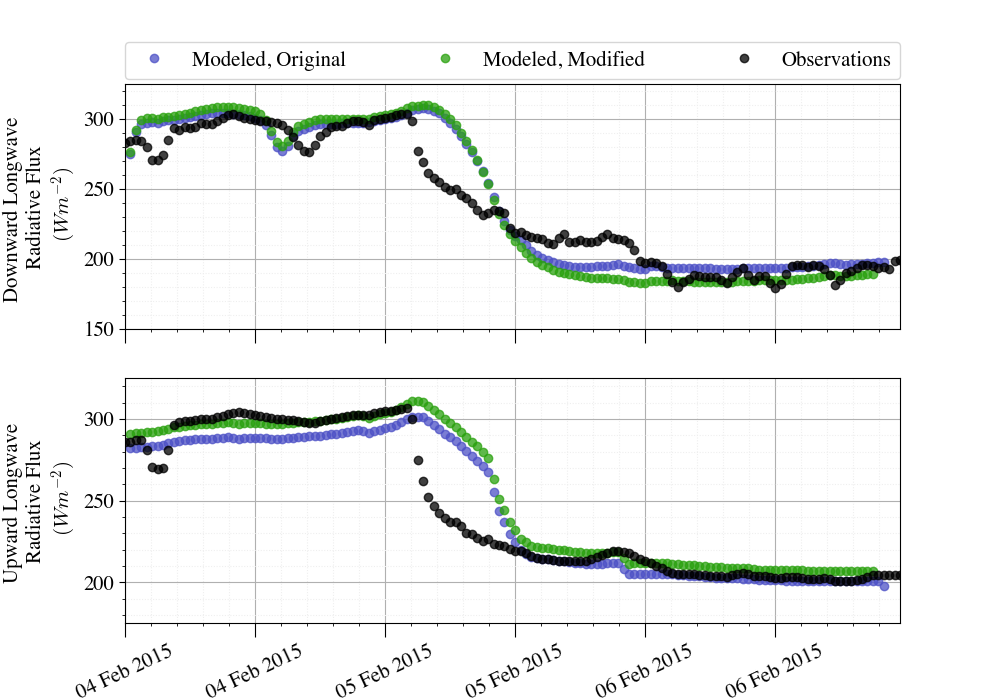
\includegraphics[width=1\linewidth]{figures/chapter6/case1_lw_sw.png}
    \caption[Idealized Case 1 - Longwave radiation.]{Upward longwave radiation (top) and downward longwave radiation (bottom) for the model with original LANDUSE.TBL values (blue), the model with modified LANDUSE.TBL values (green), and the observations (black) from 4 February to 6 February.}
    \label{fig:c1:radiative}
\end{figure}

\begin{table}[b!]
\centering
\footnotesize
\doublespacing
{
\begin{tabular}{| c | c | c | c | c | c | c | c | c |}
\hline
\rowcolor[HTML]{F3F3F3} & & \textbf{Latent} & \textbf{Sensible} & \textbf{LW Down} & \textbf{LW Up} & \textbf{SW Down} & \textbf{SW Up} \\
\hline 
\cellcolor[HTML]{F3F3F3} & \cellcolor[HTML]{F3F3F3} \textbf{Modified} & 12.13 & 	38.11	& -0.19	& 6.5 & & \\
\cellcolor[HTML]{F3F3F3}& \cellcolor[HTML]{F3F3F3} \textbf{Original} & 13.52 &	47.1	& 2.48	& -1.23 & & \\
\cellcolor[HTML]{F3F3F3}\multirow{-3}{*}{\shortstack{\textbf{Winter} \\ \textbf{Cloudy}}} & \cellcolor[HTML]{F3F3F3} \textbf{Difference} & -1.39 &	-8.99 &	-2.67 &	7.73 & & \\
\hline
\cellcolor[HTML]{F3F3F3} & \cellcolor[HTML]{F3F3F3} \textbf{Modified} & 1.6 &	-3.86 &	-54.83	& -11.69 &	111.15 &	81.96 \\
\cellcolor[HTML]{F3F3F3} & \cellcolor[HTML]{F3F3F3} \textbf{Original} & -0.2 &	-9.81 &	0.34 &	-19.14 &	50.2 &	33.21 \\
\cellcolor[HTML]{F3F3F3} \multirow{-3}{*}{\shortstack{\textbf{Spring} \\ \textbf{Cloudy}}} & \cellcolor[HTML]{F3F3F3} \textbf{Difference} & 1.8 &	5.95 &	-55.17	& -7.45	& 60.95 &	48.75 \\
\hline
\cellcolor[HTML]{F3F3F3} & \cellcolor[HTML]{F3F3F3} \textbf{Modified} & 3.98	& -2.25 &	-36.17 &	-5.58 &	50.4 &	48.41 \\
\cellcolor[HTML]{F3F3F3} & \cellcolor[HTML]{F3F3F3} \textbf{Original} & 4.81	& 0.23	& -8.15 & 	-13.31	& 13.39	& 15.04 \\
\cellcolor[HTML]{F3F3F3} \multirow{-3}{*}{\shortstack{\textbf{Spring} \\ \textbf{Clear}}} & \cellcolor[HTML]{F3F3F3} \textbf{Difference} \cellcolor[HTML]{F3F3F3} & -0.83 &	-2.48	& -28.02	& 7.73 &	37.01	& 33.37 \\
\hline
\end{tabular}}
\caption[Mean model bias for idealized WRF runs with modified LANDUSE.TBL values.]{Mean model biases ($Wm^{-2}$) for each idealized case study with both the modified (top of each case) and original (middle of each case) runs. Differences in biases (modified - original) are shown in the last row of each case labeled ``Difference." Positive differences indicate an increase in error and negative indicate a decrease in error when table modifications are implemented.}
\label{tab:wrf:meanbias}
\end{table}

The first case study period was from 4 February to the end of the day on 6 February. This was during a cloudy period in the winter and has been named the ``Winter Cloudy" case. The downward and upward latent heat fluxes can be seen in Figure \ref{fig:c1:heat}. The modeled values do not capture the timing or sharp decrease in longwave radiation on 5 February. The modifications in the LANDUSE.TBL file do not significantly impact these fluxes, but it can be seen in Table \ref{tab:meanbias} that the modifications do reduce the mean bias in the downward longwave radiation but increase the bias in the upward longwave radiation. 

\begin{figure}[h]
    \centering
    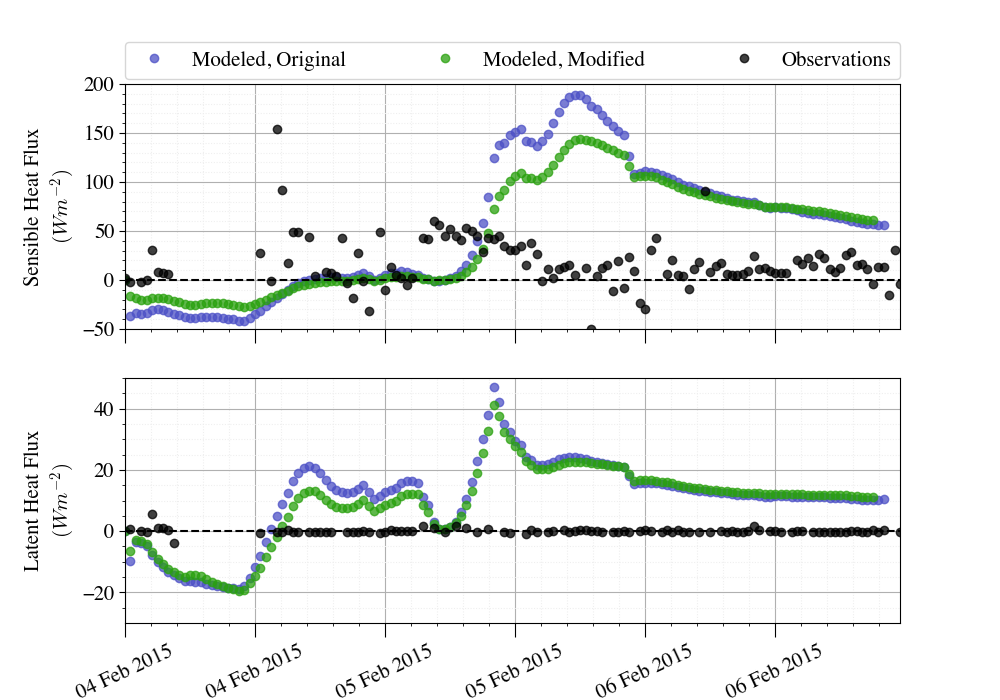
\includegraphics[width=1\linewidth]{figures/chapter6/case1_sensible_latent.png}
    \caption[Idealized Case 1 - Latent and sensible heat fluxes.]{Sensible heat flux (top) and latent heat flux (bottom) for the model with original LANDUSE.TBL values (blue), the model with modified LANDUSE.TBL values (green), and the observations (black) from 4 February to 6 February.}
    \label{fig:c1:heat}
\end{figure}

The modification in the land use table also improved latent and sensible heat flux biases. Table \ref{tab:meanbias} shows the sensible heat flux bias was reduced by almost 10 $Wm^{-2}$ in the simulations with the modified values. Latent heat flux was also improved. Figure \ref{fig:c1:heat} shows the time series of the fluxes. The modifications to the land use table do reduce the values, but they do not bring them any closer to capturing any observed patterns in the fluxes during this case.

\begin{figure}[p]
    \centering
    \vspace{-10em}
    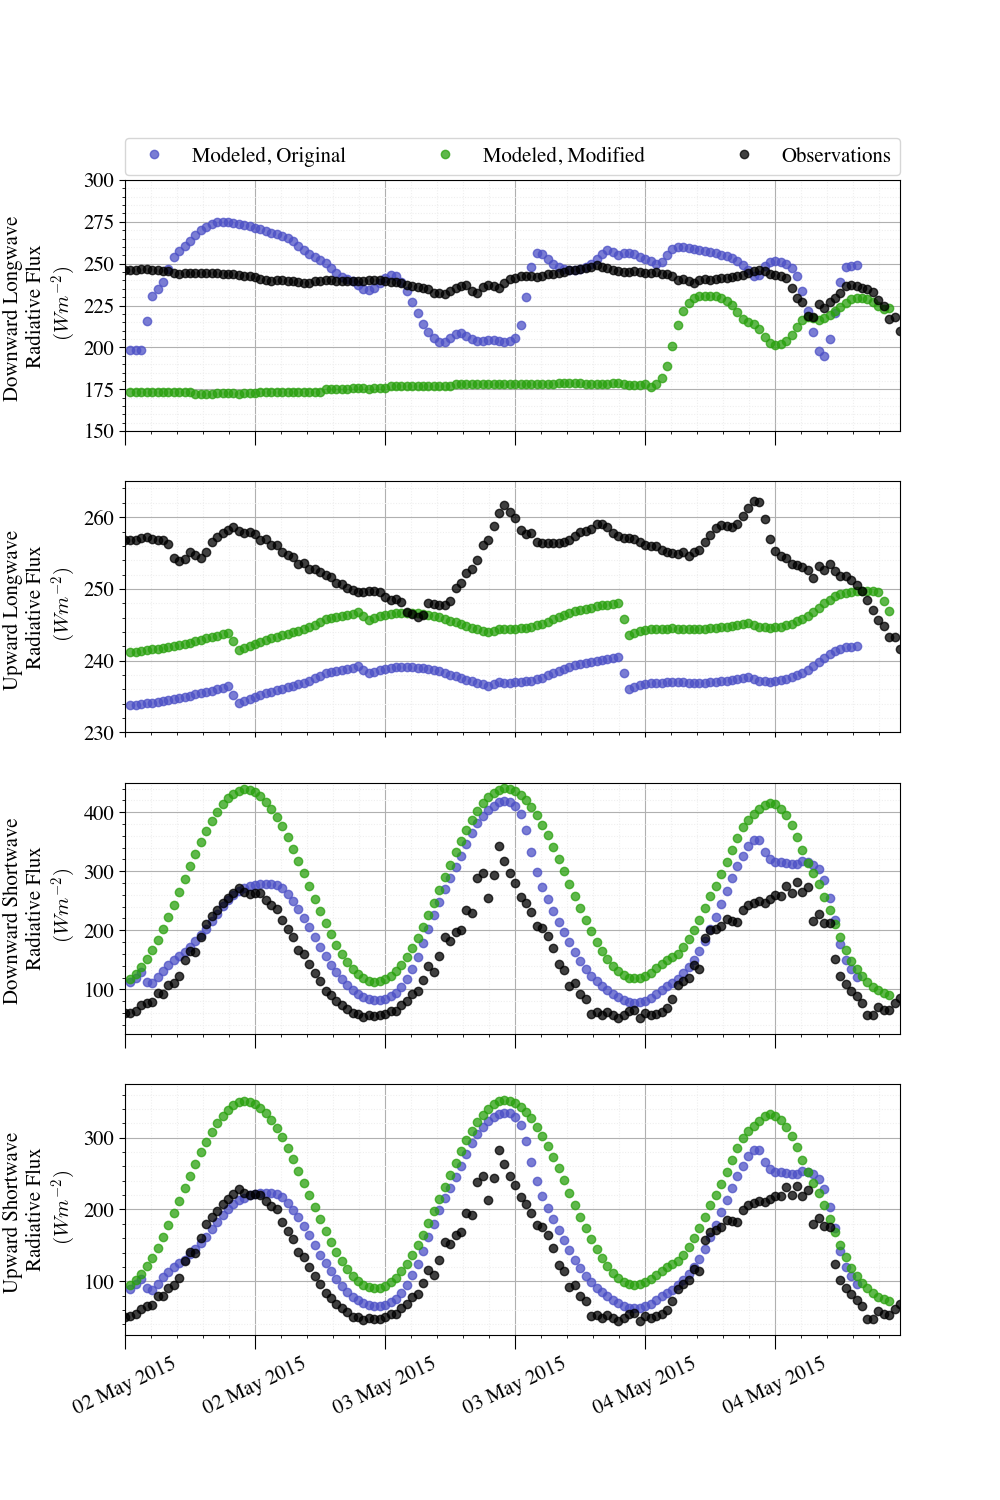
\includegraphics[width=1\linewidth]{figures/chapter6/case2_lw_sw.png}
    \caption[Idealized Case 2 - Longwave radiation.]{Upward longwave radiation (top), downward longwave radiation (second from top), upward shortwave radiation (second from bottom), and downward shortwave radiation (bottom) for the model with original LANDUSE.TBL values (blue), the model with modified LANDUSE.TBL values (green), and the observations (black) from 2 May to 4 May.}      
    \label{fig:c2:radiative}
\end{figure}

The second case study period was a cloudy period in the spring. Radiative fluxes for this period can be seen in Figure \ref{fig:c2:radiative}. At this time, the sun was rising over the N-ICE ship, so there is a shortwave component to the flux. The modified values did not do well for this case and changing the LANDUSE.TBL values removed many of the clouds during this period. While the cloud mask is not shown here, this is clear in both the longwave and shortwave radiation. The shortwave radiation (bottom panels, Figure \ref{fig:c2:radiative}) shows less radiation in the unmodified modeled results than in the modified. In fact, the unmodified results match the measurements fairly well in the shortwave. The lack of clouds in the modified simulation can also be seen in the longwave downward flux (Figure \ref{fig:c2:radiative}). These fluxes for the modified simulation are consistently much lower than those from the original runs and have little variation until the last day when the model finally begins to produce cloud cover. 

\begin{figure}[t]
    \centering
    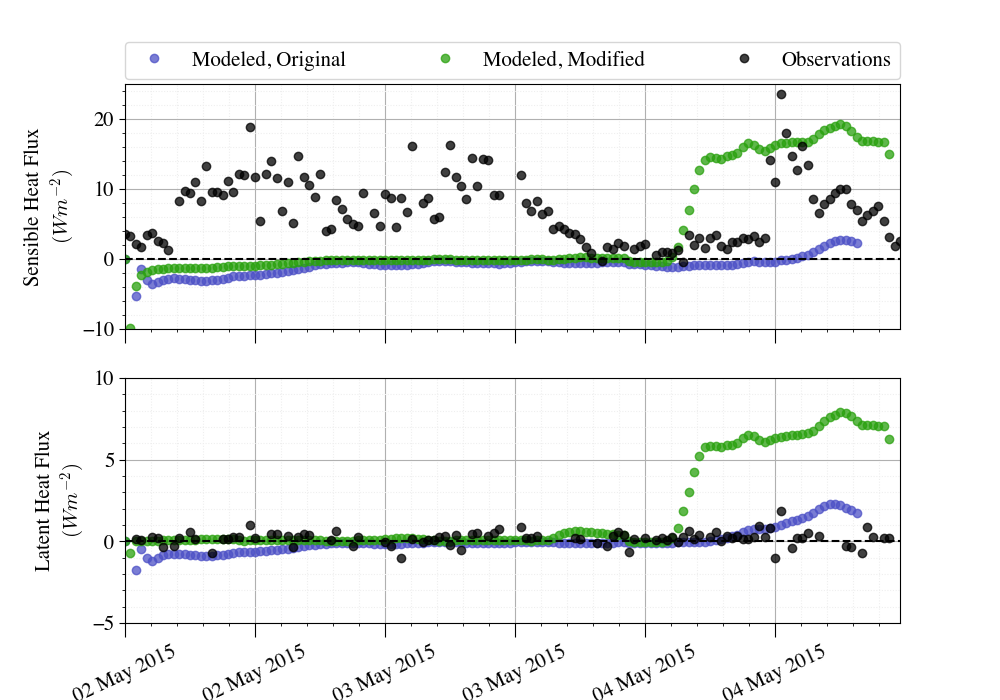
\includegraphics[width=1\linewidth]{figures/chapter6/case2_sensible_latent.png}
    \caption[Idealized Case 2 - Latent and sensible heat fluxes.]{Sensible heat flux (top) and latent heat flux (bottom) for the model with original LANDUSE.TBL values (blue), the model with modified LANDUSE.TBL values (green), and the observations (black) from 2 May to 4 May.}
    \label{fig:c2:heat}
\end{figure}

The modified LANDUSE.TBL produced higher sensible and latent heat flux values near the end of the study period (Figure \ref{fig:c2:heat}). Some increased sensible heat flux values are observed near the end of this case, and at this point, as the modified model is producing clouds and warming the air above the surface, making this the only variable and time period during this case that the modified simulation outperformed the original. Overall, mean biases (Table \ref{tab:meanbias}) were higher for the model runs using the modified values than those using the original table values.

\begin{figure}[p!]
    \centering
    \vspace{-10em}
    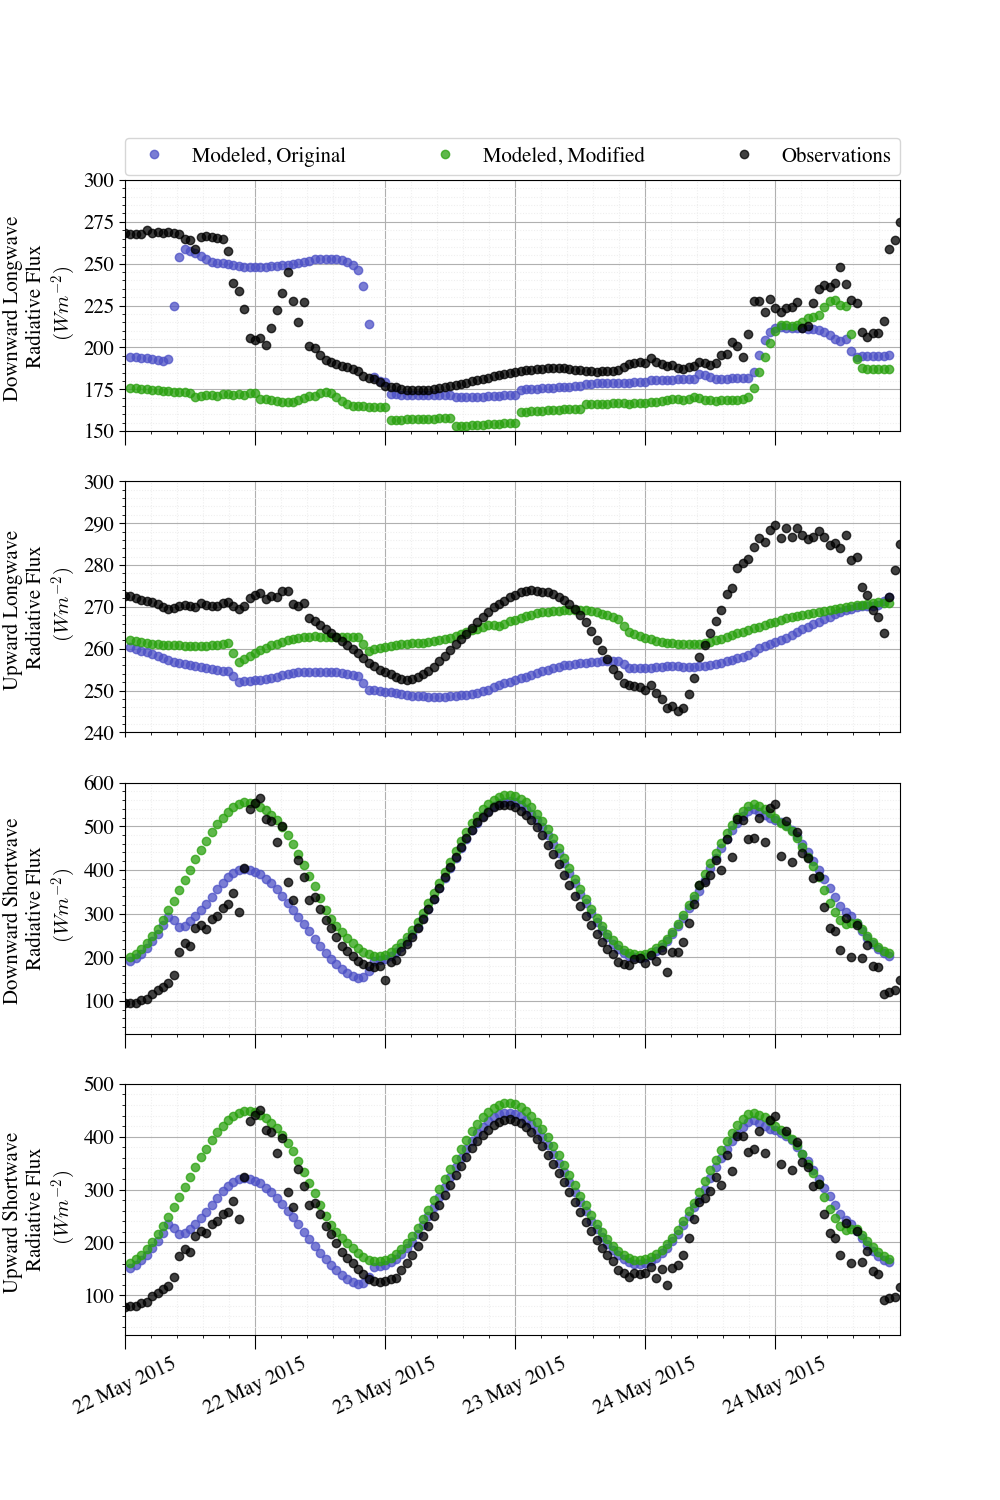
\includegraphics[width=1\linewidth]{figures/chapter6/case3_lw_sw.png}
    \caption[Idealized Case 3 - Longwave radiation.]{Upward longwave radiation (top), downward longwave radiation (second from top), upward shortwave radiation (second from bottom), and downward shortwave radiation (bottom) for the model with original LANDUSE.TBL values (blue), the model with modified LANDUSE.TBL values (green), and the observations (black) from 22 May to 24 May.}    
    \label{fig:c3:radiative}
\end{figure}

The last case study period is from 22 May to 24 May, when the N-ICE field site experienced 24 hours of cloudless skies. This 24-hour period was captured well by both the modified and unmodified simulations in the shortwave (Figure \ref{fig:c3:radiative}, bottom panels) but the day prior had some disagreement. Again, the modified simulation produced fewer clouds than those produced by the original simulations. This time, however, it matches the observations better, as the original simulation did not produce clear-sky conditions early enough in the case. The same issues can be seen with longwave radiation. Upward longwave radiation (Figure \ref{fig:c3:heat}, top) is overestimated by the original simulation for the first 24 hours of the case as the model produces clouds for too long into the evening on 22 May. The unmodified, however, does not produce enough downward longwave radiation, as this simulation did not produce enough clouds early enough. The original simulations produced lower biases for both components of shortwave radiation and the downward component of longwave radiation. Upward longwave radiation, however, had a lower bias in the modified simulation results, as the surface warmed. 

\begin{figure}[h]
    \centering
    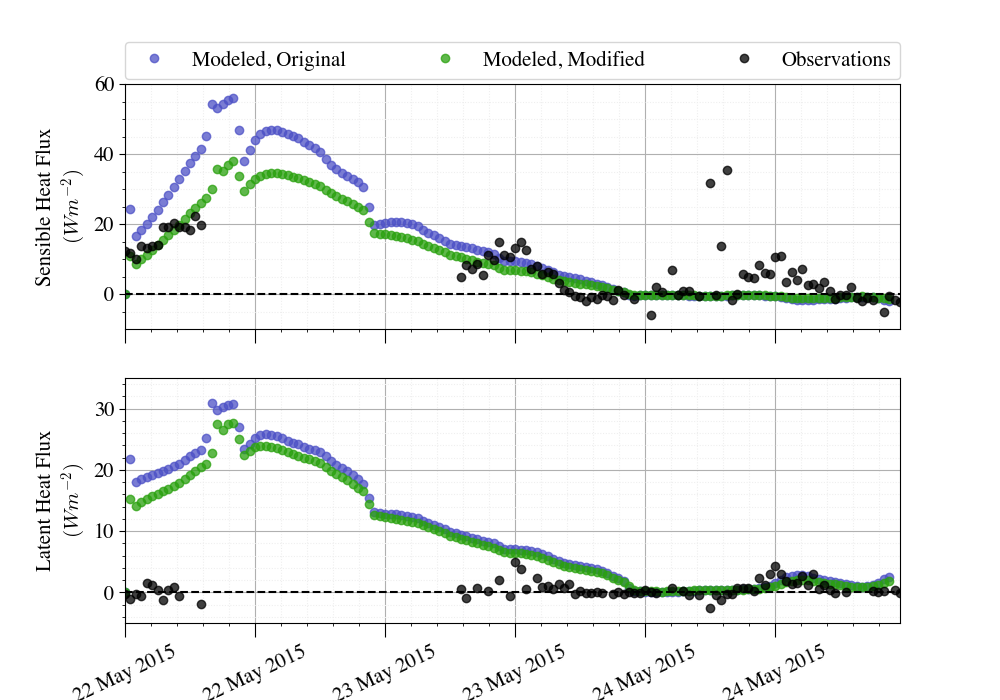
\includegraphics[width=1\linewidth]{figures/chapter6/case3_sensible_latent.png}
    \caption[Idealized Case 3 - Latent and sensible heat fluxes.]{Sensible heat flux (top) and latent heat flux (bottom) for the model with original LANDUSE.TBL values (blue), the model with modified LANDUSE.TBL values (green), and the observations (black) from 22 May to 24 May.}
    \label{fig:c3:heat}
\end{figure}

Latent and sensible heat flux values (Figure \ref{fig:c3:heat}) were similar between the two model runs past the first 24 hours. They did differ during the first day when the models had disagreements about the cloud cover. The model originally overestimated these fluxes during this time period, so even a small decrease in these values could be an improvement. Table \ref{tab:meanbias} shows that the latent heat flux bias decreased by almost 1 $Wm^{-2}$ with the modifications, but the sensible heat flux bias increased. 

\subsection{Turbulent Flux Equations}
Throughout the entire field expedition, the WRF offline calculation did a surprisingly good job of replicating the sensible heat flux observations. Figure \ref{fig:flux:sensible} shows the observations in black and the WRF offline calculation in magenta. It is often hard to see the modeled values in the time series because they are so close to the observations that many of the points overlap each other, and they create a well-defined 1:1 line on the scatter plot. This indicates that errors in estimating the sensible heat flux are likely due to the errors in values being calculated schemes outside of the SL scheme and LSM. 

\begin{figure}[t!]
    \centering
    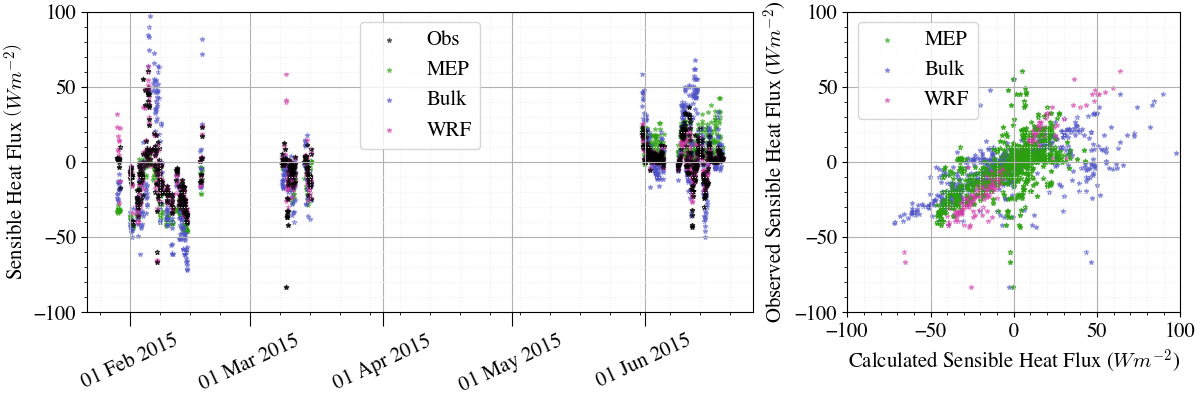
\includegraphics[width=1\linewidth]{figures/chapter6/sensible_wrf.png}
    \caption[Sensible heat flux observed at N-ICE and calculated from Polar WRF offline translated code.]{Sensible heat flux observed at N-ICE (black) and calculated from Polar WRF offline translated code (magenta), with the MEP equation (green) and with the bulk equation (blue). scatter plot (right) shows relationships between observed and calculated values shown in the time series (left).}
    \label{fig:flux:sensible}
\end{figure}
\begin{figure}[b!]
    \centering
    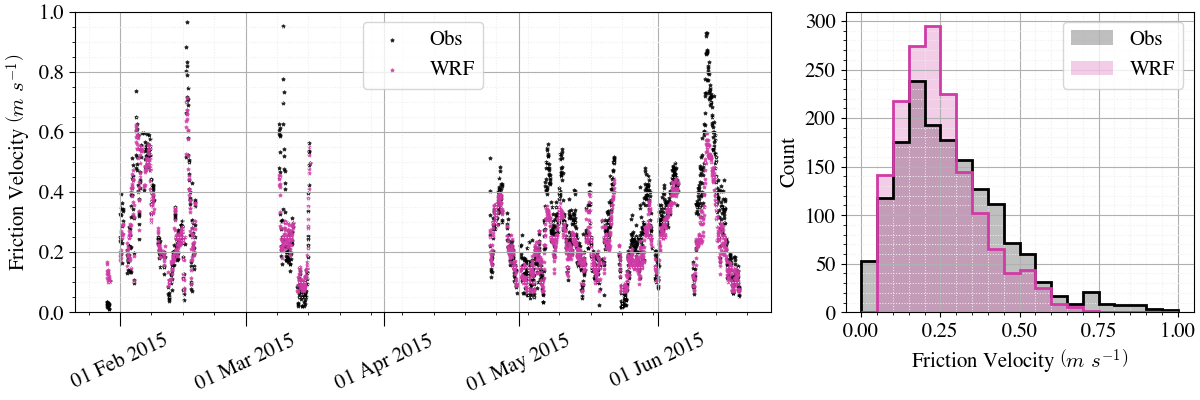
\includegraphics[width=1\linewidth]{figures/chapter6/ustar_wrf.png}
    \caption[Friction velocity observed at N-ICE and calculated from Polar WRF offline translated code.]{Friction velocity observed at N-ICE (black) and calculated from Polar WRF offline translated code (magenta).}
    \label{fig:flux:ustar}
\end{figure}

The WRF equation depends heavily on the friction velocity value, which is shown in Figure \ref{fig:flux:ustar}. The observed friction velocity has been calculated by the EddyPro software, and the WRF was calculated using the Polar WRF offline code using equations \ref{eq:wrf:ustar}. While WRF produces slightly smaller values of friction velocity, it is still fairly accurate throughout the entire observation period. 

\begin{figure}[t]
    \centering
    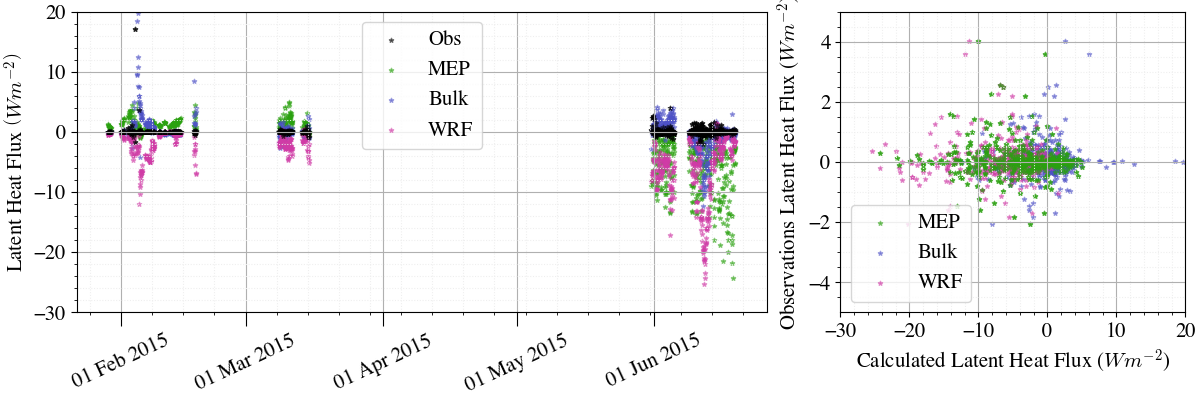
\includegraphics[width=1\linewidth]{figures/chapter6/latent_wrf.png}
    \caption[Latent heat flux observed at N-ICE and calculated from Polar WRF offline translated code.]{Latent heat flux observed at N-ICE (black) and calculated from Polar WRF offline translated code (magenta), with the MEP equation (green) and with the bulk equation (blue). Scatter plot (right) shows relationships between observed and calculated values shown in the time series (left). Note that the y-axis (observations) in the scatter plot is scaled from -5 to 5 $Wm^{-2}$ to capture the low values observed at N-ICE.}
    \label{fig:flux:latent}
\end{figure}

The results of the latent heat flux calculations (Figure \ref{fig:flux:latent}) do not match the observations anywhere near as well as the sensible heat flux calculations. The latent heat flux values at N-ICE were very small, and because of this, the y-axis on the scatter plot in Figure \ref{fig:flux:latent} has been reduced to -5 to 5 $Wm^{-2}$. All ways of calculating latent heat flux result in large errors, and none are able to accurately replicate the small values observed. Particularly in the summer, all equations gave largely negative latent heat flux values, but observations remained small.

\section{Conclusions}
Slight improvements to the WRF model performance can be made by using the appropriate surface properties for thin, first-year sea ice. However, these modifications provide slight increases in model performance but are not the solution to the large discrepancies (compared to N-ICE observations) in the turbulent heat fluxes seen in Chapter 3. Surface albedo, emissivity, and surface roughness can be adjusted to reduce the differences between the model and N-ICE observations. When turbulent flux equations were coded separately (and run ``offline") from the model using the measured radiative fluxes, they produced results very close to observations. While further improvements are likely possible, the sensitivity studies performed here show that most of the error within Polar WRF (shown in Chapter 3) can be attributed to the inaccurate cloud microphysics (CM) schemes described in Chapter 4. 

